Wenn eine Anwendung entwickelt werden soll, ist die Wahl des richtigen Frameworks oder auch der Programmiersprache eine wichtige Entscheidung für ein Projekt. Viele Entscheidungen können im Verlauf der Entwicklung noch abgeändert werden, aber um eine derartige Entscheidung zu ändern, müssen Teile der Anwendung oder auch der komplette Quellcode neu geschrieben werden. Neben Unsicherheiten bei der richtigen Wahl, erscheinen regelmäßig Artikel, die über neue Standards in der App-Entwicklung informieren wollen. So ist eine derartig wichtige Entscheidung oft sehr schwierig.

Da Anwendungen meistens nicht nur auf einem Gerätetyp, sondern allen Nutzern auf den verschiedensten Plattformen zur Verfügung stehen sollen, hat diese Entscheidung noch einmal eine größere Bedeutung, da sie eng verbunden mit den Kosten der Entwicklung und dem Nutzungserlebnis ist.

In Zeiten der Heimcomputer und des stetig wachsenden Internets war der einfachste Weg eine Webseite zu entwickeln, die über den Browser der genutzten Geräte aufgerufen werden konnte. Mit der Ära der Smartphones änderte sich dies jedoch. So waren anfänglich Webapplikationen entweder nicht für die Nutzung auf derartige Geräte mit einer Toucheingabe und kleineren Bildschirmen angepasst oder es musste eine eigene mobile Version für diese entwickelt werden\cite{Bryant2012}.

Die Nutzung von Smartphones ermöglichte allerdings die Nutzung weiterer Funktionalitäten, wie Kamera, Bluetooth oder GPS-Daten. Deshalb wurde vermehrt auf die Entwicklung einer speziellen App für Smartphones gesetzt. Sie wurden traditionell nativ mit Objectiv-C, beziehungsweise Swift, für iOS und Java beziehungsweise Kotlin, für Android entwickelt \cite{ELKASSAS2017163}, \cite{researchgate_thomas}. Durch die Programmierung mit Hilfe der nativen Programmiersprachen, entstehen für die einzelnen Plattformen gut nutzbare Anwendungen \cite{researchgate_thomas}.

Durch den Wunsch nach einer Multi-Plattform-Anwendung, also einer Anwendung, die für mehrere Plattformen veröffentlicht werden soll, muss bei der nativen Entwicklung für jede Plattform eine eigene Applikation in der jeweiligen Programmiersprache geschrieben werden. Dadurch entsteht ein hoher Aufwand und die Kosten multiplizieren sich mit der Zahl der abzudeckenden Plattformen.

Deswegen wurden bereits früh sogenannte Cross-Plattform-Technologien entwickelt, die es ermöglichen, mit einem geteilten Code, so viele Plattformen wie möglich abzudecken. So erschien etwa 2008 PhoneGap. Es war ein Open-Source Framework zur Entwicklung von hybriden mobilen Applikationen, die mit Hilfe von HTML, CSS und JavaScript implementiert wurden. PhoneGap und sein Nachfolger Cordova waren einige Zeit sehr beliebt in diesem Bereich und hatten 2019 zusammen einen Marktanteil von etwa 40\% unter den Cross-Plattform-Frameworks \cite{statist_CP_Framework}.

Trotz des geringeren Aufwandes und den damit geringeren Kosten, werden dennoch viele Applikationen immer noch nativ entwickelt. So ergab eine interne Untersuchung der Firma ScanBotSDK\footnote{\label{scanbot_footnote}\url{https://scanbot.io/de/blog/native-apps-vs-cross-platform/}}, dass 2019, 57\% ihrer Nutzer native Applikationen entwickelten, obwohl ihr Produkt ebenso für viele der gängigen Cross-Plattform-Frameworks zur Verfügung steht.

Ein Grund für Unsicherheit in diesem Bereich sind oft auch negative Erfahrungsberichte von Firmen, die einen Umstieg von einer nativen Applikation zu einer Cross-Plattform-Applikation versuchten. So etwa auch Airbnb \cite{Airbnb_react_goals}. Sie nutzten das von Facebook mitentwickelte Framework React Native\footnote{\url{https://reactnative.dev/}}. Dieses Framework hatte 2019 hatte einen Marktanteil von 42\% \cite{statist_CP_Framework}. 
\break
Airbnbs Ziele waren einfach \cite{statist_CP_Framework}:
\begin{enumerate}%This could be compactenum or inparaenum see paralist dokumentation%
    \item schnelleres entwickeln
    \item die gleiche Codequalität beibehalten
    \item nur noch eine Codebasis
    \item die Entwicklungsabläufe verbessern
\end{enumerate}
\nointerlineskip
Jedoch traten während der Entwicklung mit React Native einige technische Probleme auf. So musste beispielsweise eine eigene Version des genutzten Frameworks erstellt werden, um notwendige Änderungen einzubauen. Dies erschwerte es jedoch, Updates des Frameworks zu integrieren \cite{Airbnb_technology}. Die Entwickler von Airbnb erkannten, dass sie ihre Ziele nicht einhalten konnten und kehrten 2018 wieder zu einem nativen Ansatz zurück.

Wegen Beispielen wie diesen, sind App-Entwickler oft skeptisch gegenüber neuen Ansätzen, da ein Umstieg häufig mit großen Änderungen, hohen Investitionen und einer Einarbeitungszeit verbunden sind \cite{medium_Lehtimäki}. Dennoch nimmt die Zahl der Cross-Plattform-Entwicklungen in den letzten Jahren zu. 
So ergab die Untersuchung von ScanBotSDK\footnoteref{scanbot_footnote}, dass im Jahre 2021, gerade einmal zwei Jahre später, 58\% Cross-Plattform-Lösungen nutzten. Diese Zahl stützt auch eine Untersuchung von Jetbrains \cite{JetBrains_miscellaneous_2021}. Diese ergab, dass 2021 53\% aller App Entwickler, Cross-Plattform-Technologien nutzten.

\begin{figure}[ht]
  \centering
  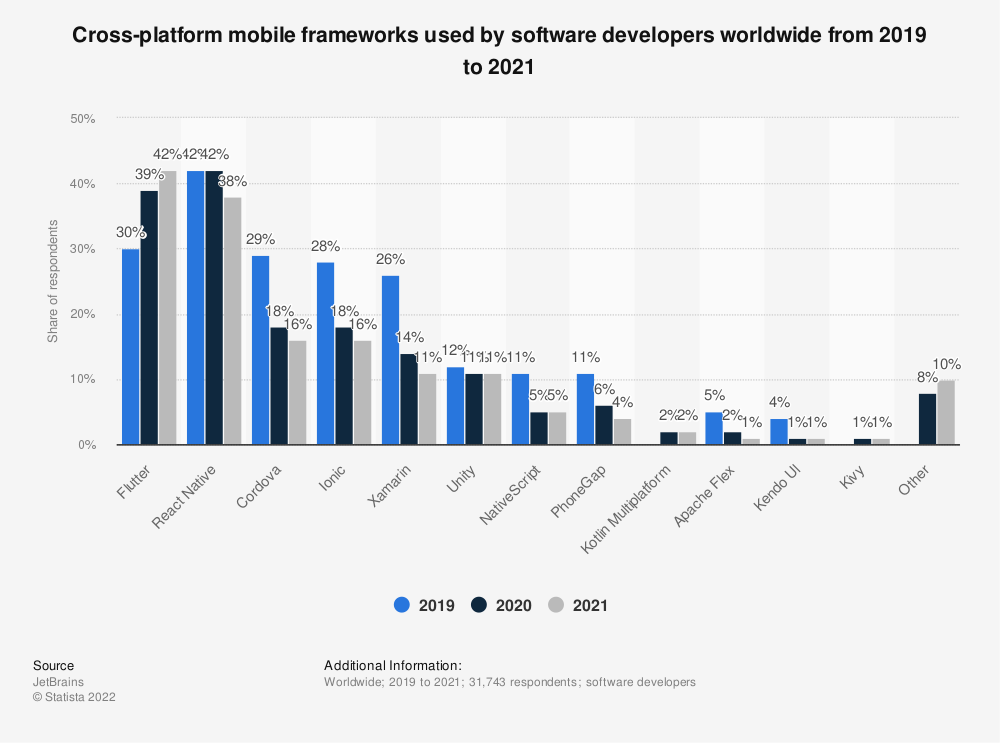
\includegraphics[width=15cm,keepaspectratio]{images/cross-platform-mobile-frameworks.png} 
  \caption[Statistik Cross-Plattform-Frameworks]{Cross-Plattform-Frameworks 2019-2021 \cite{statist_CP_Framework}}
  \label{fig:statista_cross_plattform}
\end{figure}

Diese Zahl dürfte in den nächsten Jahren weiter steigen. Einen Grund dafür bieten unter anderem auch neu entstandene Frameworks. In Abbildung \ref{fig:statista_cross_plattform} ist eine Statistik zu sehen, die die Verteilung von verschiedenen Cross-Plattform-Entwicklungstechnologien zwischen 2019 und 2021 zeigt. Sie verdeutlicht wie schnell sich die Verteilung von Cross-Platform Frameworks ändern kann. Flutter ist dafür ein gutes Beispiel. Es ist ein Framework das erst 2017 auf den Markt gekommen ist und innerhalb von gerade einmal 4 Jahren einen Marktanteil von 42\% erreicht hat. Von manchen wird es als der neue Standard angesehen und einige Unternehmen steigen auf eine Entwicklung mit Flutter um \cite{flutter_move_to}, \cite{flutter_move_to_dart}. 

Jedoch gibt es auch weiterhin Entwickler, die nur nativ entwickeln. So etwa die App-Agentur Number42, mit der diese Arbeit in Zusammenarbeit entstanden ist. Sie entwickeln Web- und mobile Applikationen. Alle der dort entwickelten mobilen Applikationen sind mit den nativen Programmiersprachen geschrieben. Einerseits entwickeln sich auch die nativen Programmiersprachen stetig weiter und erhalten Änderungen, die eine Entwicklung vereinfachen und beschleunigen. Andererseits gibt es auch Projekte, bei denen lediglich eine Plattform benötigt wird, da sie nur auf Geräten des Unternehmens ausgeführt werden sollen und diese beispielsweise nur Smartphones der Firma Apple nutzen. Deswegen ist auch dieser Ansatz nicht von der Hand zu weisen und es kann durchaus sinnvoll sein, neue Apps weiterhin nativ zu entwickeln.

\section{Beitrag dieser Arbeit}
Der Inhalt dieser Arbeit ist die Beschreibung vier verschiedener Implementierungen und deren Vergleich anhand unterschiedlicher Kriterien. Dafür werden Daten aus der Implementierung, Dokumentationen und anderen Quellen gesammelt und verglichen.
Um ein einheitliches Verständnis für die verschiedenen Entwicklungsansätze zu erhalten, werden diese zunächst vorgestellt. Dies ist nötig, da es einige verschiedene Einordnungen in wissenschaftlichen Arbeiten gibt.
Als Implementierungen werden eine native Applikation mit Kotlin, eine hybride Applikation mit Kotlin, eine cross-kompilierte Applikation mit Flutter und eine gemischte Implementierung mit Flutter vorgestellt. 
Weiterhin werden die vorgestellten Implementierungen auf die Kriterien Performance und Entwicklung, Entwicklergemeinschaft, Entwicklungsdauer, Benutzeroberfläche (UI) und Funktionalität untersucht.
Dabei konnte unter anderem ein deutlich geringerer Programmmieraufwand bei den Cross-Plattform-Implementierungen im Vergleich zu der nativen Implementierung festgestellt werden. In Sachen Performance schnitt zwar die native Applikation am besten ab, jedoch war der Unterschied vor allem zu der cross-kompilierte Lösung nicht erheblich. Die cross-kompilierte Applikation konnte beispielsweise durch eine schnelle Renderzeit oder umfassenden Plattformunterstützung zeigen, dass sie eine Alternative zu den nativen Applikationen darstellt. Insgesamt wurde jedoch festgestellt, dass es bei einer möglichen Entscheidung vor allem auf die Anforderungen und Begebenheiten eines Projektes ankommt.

\section{Aufbau der Arbeit}
In Kapitel 2 werden zunächst verwandte Arbeiten vorgestellt, während in Kapitel 3 die verschiedenen Applikationsklassen, einige Begriffe und die Implementierungen vorgestellt und die Arbeit abgegrenzt wird.
Danach werden in Kapitel 4 die verschiedenen Implementierungen und einige der während der Entwicklung gewonnenen Erkenntnisse erläutert. Dabei soll auch auf Stärken und Schwächen der einzelnen Implementierungen eingegangen werden, die während der Implementierung und Recherche aufgefallen sind.
In Kapitel 5 soll anschließend eine Auswertung der Implementierungen anhand einiger Kriterien stattfinden und mit weiteren Erklärungen und Vergleichen, eine Einordnung der verschiedenen Ansätze stattfinden. Abschließend soll in Kapitel 6 ein Fazit gezogen und ein Ausblick auf weitere Themen gegeben werden.